% This thesis template is based on the personal template of Felix Moebius. Thanks, Felix!
% It has been extended and modified by Tobias Pfandzelter at the Scalable Software Systems group of TU Berlin.
% It is licensed under the terms of the MIT license, meaning you are free to use it however you see fit but we accept no liability.
% Good luck writing your thesis!

\documentclass[a4paper, 11pt]{article}

\usepackage[utf8x]{inputenc}
\usepackage[T1]{fontenc}
\usepackage{fix-cm}

\usepackage[a4paper, margin=3cm]{geometry}
\usepackage[titletoc, title]{appendix}

\usepackage{color}
\usepackage{booktabs}
\usepackage[all]{nowidow}
\usepackage[dvipsnames]{xcolor}
\usepackage[hidelinks]{hyperref}
\usepackage{acronym}
\usepackage{graphicx}
\usepackage{url}
\usepackage{titlesec}
\usepackage{csquotes}

\usepackage{transparent}
\usepackage{eso-pic}
\usepackage[section]{placeins}
\usepackage{setspace}
\usepackage{parskip}
\usepackage{subcaption}
\usepackage{color,soul}

\renewcommand\thefigure{%
\thesection.\arabic{figure}}
\renewcommand\thesubfigure{%
\thesection.\arabic{figure}.\arabic{subfigure}}
\renewcommand\thetable{%
\thesection.\arabic{table}}

\usepackage[main=english, ngerman]{babel}

% we use the cleveref package to refer to figures, sections, etc.
% instead of "Figure~\ref{fig:example}", write only "\cref{fig:example}" and the word "Figure" (or table, etc) will be inserted normally
\usepackage[noabbrev,capitalise]{cleveref}

\usepackage[
    maxbibnames=99,
    style=alphabetic,
    url=false,
    backend=bibtex8,
    sortcites=true,
]{biblatex}
\addbibresource{refs.bib}
\DeclareFieldFormat[online]{urldate}{Last accessed: #1}
\DeclareFieldFormat{eprint}{arXiv: \href{https://arxiv.org/abs/#1}{#1}}
\DeclareFieldFormat[report]{title}{``#1''}


\newcommand{\projectTitle}{Exploring Datastore Access Latency across AWS Compute Services}
\newcommand{\thesisType}{Bachelor's Thesis}
\newcommand{\authors}{Bhupendra Singh}
\newcommand{\matrikel}{464877}
\newcommand{\authorEmail}{\href{mailto:b.singh@campus.tu-berlin.de}{b.singh@campus.tu-berlin.de}}
\newcommand{\examinera}{Prof.~Dr.-Ing.~David Bermbach}
\newcommand{\examinerb}{Prof.~Dr.~habil.~Odej Kao}
\newcommand{\supervisor}{Trever Schirmer}

\newcommand{\projectYear}{2024}
\newcommand{\facultyName}{Fakultät Elektrotechnik und Informatik}
\newcommand{\departmentName}{Fachgebiet Scalable Software Systems}

\begin{document}
{\sffamily\color{white}\raggedright\setlength{\parindent}{0cm}\large\onehalfspacing
\AddToShipoutPicture*{
    \put(-4,0){
        \parbox[b][\paperheight]{\paperwidth}{%
            \vfill
            \centering
            
\includegraphics[width=\paperwidth]{title.pdf}%
            \vfill
        }
    }
}

\vfill
\vspace*{5cm}

{\huge\textbf{\projectTitle}\par}
\vspace*{0.5cm}
\textbf{\thesisType}      \\
\vspace*{2cm}
\textbf{Author}               \\
\authors              \\
\matrikel                     \\
\authorEmail                  \\
\vspace*{1cm}
\textbf{Advisor}              \\
\supervisor                   \\
\vspace*{1cm}
\textbf{Examiners}            \\
\examinera                    \\
\examinerb

\vfill

\textbf{Technische Universit\"at Berlin, \projectYear} \\
\small{\facultyName \\
    \departmentName}
\vspace{1cm}
}

\thispagestyle{empty}
\clearpage

\vspace*{\fill}
\begin{centering}
    {\huge\textbf{\projectTitle}\par}
    \vspace{1cm}
    \large{\thesisType}\\
    \vspace{1cm}
    Submitted by:\\
    \authors\\
    \matrikel                     \\
    \authorEmail                  \\
    \vspace{1cm}
    Technische Universit\"at Berlin\\
    \facultyName \\
    \departmentName \\
    \vspace{1cm}
    \projectYear\\

\end{centering}

\vspace*{\fill}
\thispagestyle{empty}
\clearpage

\vspace*{\fill}
{
    % briefly set the footnote to symbols for this disclaimer
    \renewcommand*{\thefootnote}{\fnsymbol{footnote}}
    \noindent
    \begin{otherlanguage}
        {ngerman}
        Hiermit versichere ich, dass ich die vorliegende Arbeit eigenständig ohne Hilfe Dritter und ausschließlich unter Verwendung der aufgeführten Quellen und Hilfsmittel angefertigt habe.
        Alle Stellen die den benutzten Quellen und Hilfsmitteln unverändert oder sinngemäß entnommen sind, habe ich als solche kenntlich gemacht.

        Sofern generische KI-Tools verwendet wurden, habe ich Produktnamen, Hersteller, die jeweils verwendete Softwareversion und die jeweiligen Einsatzzwecke (z.~B.~sprachliche Überprüfung und Verbesserung der Texte, systematische Recherche) benannt.
        Ich verantworte die Auswahl, die Übernahme und sämtliche Ergebnisse des von mir verwendeten KI-generierten Outputs vollumfänglich selbst.

        Die Satzung zur Sicherung guter wissenschaftlicher Praxis an der TU Berlin vom 8. März 2017\footnote{\url{https://www.static.tu.berlin/fileadmin/www/10000060/FSC/Promotion___Habilitation/Dokumente/Grundsaetze_gute_wissenschaftliche_Praxis_2017.pdf}} habe ich zur Kenntnis genommen.

        Ich erkläre weiterhin, dass ich die Arbeit in gleicher oder ähnlicher Form noch keiner anderen Prüfungsbehörde vorgelegt habe.
        \vskip 2cm
        \begin{tabular}{@{}p{.5in}p{4in}@{}}
             & \hrulefill                              \\
             & (Unterschrift) \authors, Berlin, \today \\
        \end{tabular}

    \end{otherlanguage}
    % reset footnote styling for the rest of the thesis
    \renewcommand*{\thefootnote}{\arabic{footnote}}
    \setcounter{footnote}{0}
}

\vspace*{\fill}
\thispagestyle{empty}
\clearpage


\newpage

\section*{Abstract}
Cloud computing has become essential for modern applications, offering scalable and flexible services. Amazon Web Services (AWS) is a leading provider, yet little empirical data exists on how its compute and datastore services interact in terms of access latency. This thesis benchmarks access latency between EC2 and Lambda compute services paired with RDS, DynamoDB, and S3 datastores under constant and burst workloads. The results reveal that EC2-based pairs consistently deliver lower latency and more stable performance compared to Lambda-based pairs, which show greater variability. These insights can guide cloud architects in designing latency-sensitive applications. However, limitations such as simplified configurations, AWS Free Tier constraints, and single-region testing highlight the need for further studies to explore more complex and distributed scenarios. This thesis provides initial foundational insights that can serve as a basis for further exploration and development.

% GERMAN
\clearpage
\begin{otherlanguage}
    {ngerman}
    \section*{Kurzfassung}
    Cloud-Computing ist unverzichtbar für moderne Anwendungen geworden, da es skalierbare und flexible Dienste bietet. Amazon Web Services (AWS) ist ein führender Anbieter, jedoch es gibt nur wenige empirische Daten darüber, wie seine Compute- und Datenspeicherdienste in Bezug auf Zugriffslatenz zusammenwirken. Diese Arbeit benchmarkt die Zugriffslatenz zwischen den Compute-Diensten EC2 und Lambda in Kombination mit den Datenspeicherdiensten RDS, DynamoDB und S3 unter konstanten und variierenden Arbeitslasten. Die Ergebnisse zeigen, dass EC2-basierte Paare konsistent niedrigere Latenzen und eine stabilere Leistung liefern als Lambda-basierte Paare, die größere Schwankungen aufweisen. Diese Erkenntnisse können Cloud-Architekten dabei unterstützen, latenzsensible Anwendungen zu entwickeln. Einschränkungen wie vereinfachte Konfigurationen, die Beschränkungen des AWS Free Tiers und die Begrenzung auf eine einzige Region verdeutlichen jedoch die Notwendigkeit weiterer Studien, um komplexere und verteilte Szenarien zu untersuchen. Diese Arbeit liefert erste grundlegende Einblicke, die als Basis für weitere Untersuchungen und Entwicklungen dienen können.
\end{otherlanguage}

\clearpage

\tableofcontents

\section{Introduction}
\label{cha:intro}

% BACKGROUND AND MOTIVATION
Cloud computing delivers on-demand resources like servers, storage, and databases via the Internet, eliminating the need for physical infrastructure and enabling flexibility and scalability. Its adoption has surged in the past decade and Amazon Web Services (AWS) has emerged as a leader and pioneer of various cloud models. AWS maintains 31\% market share driven by its innovation and broad service portfolio \cite{web_richter_cloud_market}.

% PROBLEM STATEMENT
Applications in cloud environments typically consist of compute and datastore service instances that interact frequently, therefore latency between these services significantly influences the overall performance and user experience of the application \cite{atricle_dean_tail,book_popescu_netlat}. AWS provides performance insights for its datastore services from both the service-side and client-side perspectives. The service-side perspective evaluates how efficiently the datastore performs internally. In contrast, the client-side perspective focuses on the time taken for a client to receive a response after submitting a query. However, it remains unclear how client-side latency varies across different AWS compute services.

% THESIS CONTRIBUTION
Prominent AWS compute services include (1) Elastic Cloud Compute (EC2), which offers customizable virtual machines for consistent performance and long-running workloads, and (2) Lambda, a serverless, event-driven service ideal for short tasks and automatic scaling. Popular AWS datastore services include (1) Relational Database Service (RDS), which provides managed SQL databases for structured data, (2) DynamoDB, a serverless NoSQL database for high-scale, low-latency use cases, and (3) Simple Storage Service (S3), a distributed object storage service for unstructured data.

In this thesis, we benchmark access latency between the above AWS compute and datastore services to examine how the choice of compute service affects latency dynamics with datastores, such as whether an EC2-RDS pair outperforms a Lambda-RDS pair. The results consistently show that EC2-based pairs outperform Lambda-based pairs by small margins. This thesis provides insights for cloud architects and application developers to optimize AWS compute and datastore service selection based on access latency, supporting decision-making for latency-sensitive applications and improving cloud architecture and cost-efficiency.

We therefore make the following contributions in this thesis:
\begin{enumerate}
	\item We address the identified knowledge gap by proposing a benchmark in \cref{cha:approach}.
	\item We evaluate the proposed approach through experimentation in \cref{cha:implementation}.
	\item We present and interpret our results in \cref{cha:results}.
	\item We discuss our observations, possible causes, and limitations in \cref{cha:discuss}.
\end{enumerate}

\clearpage
\section{Background}
\label{cha:background}

TODO (Define RDS, DynamoDB, S3, EC2, Lambda, k6, terraform)
\clearpage
\section{Benchmark Design}
\label{cha:approach}

In this section, we present our approach to benchmark AWS compute and datastore service pairs, while addressing requirements and challenges discussed in \cref{cha:background}. Affordability is a major requirement in this thesis, as the whole experiment is conducted within the limits of AWS Free Tier\footcite{https://aws.amazon.com/free/}. This influences design and implementation decisions while necessitating trade-offs with other requirements.

\cref{cha:intro,cha:background} highlight the importance of access latency in applications and it is the primary metric of interest in this thesis. To isolate access latency, we focus on read-only operations between compute and datastore services, to avoid locking and transactional overheads in writes. Queries are kept simple, database tables, and object files minimal to reduce querying and data transmission overhead. While mixed read-write workloads, larger databases, and complex queries reflect real-world scenarios, simple read-only benchmarks can provide initial baseline latency performance. Additionally, focusing on reads is cost-effective, as services like S3 offer significantly more free-tier reads compared to writes.

We evaluate and compare six pairs of prominent AWS compute and datastore services for access latency: (1) EC2-RDS, (2) EC2-DynamoDB, (3) EC2-S3, (4) Lambda-RDS, (5) Lambda-DynamoDB, and (6) Lambda-S3. Each benchmarking run involves two primary components: (1) a pre-loaded datastore serving as the System Under Test (SUT) and (2) a compute instance which generates workload on the SUT and collects access latency data. For simplicity, we refer to the datastore as SUT and the compute instance as workload generator in this thesis. However, in our context, a compute instance and a datastore together constitute one SUT, as we are not particularly testing the datastores.

To address relevance, we employ open workload model, due to the reasons discussed in \cref{elems_of_bench} and evaluate each pair under two distinct workload types: constant and burst. Under constant workload, the reads per second (RPS) remain stable throughout the benchmarking run. A burst workload, on the other hand, simulates sudden spikes in RPS, reflecting real-world scenarios where workload can be unpredictable. This allows us to observe how each pair performs under steady load and how they respond to fluctuating, high-demand conditions. To address repeatability we evaluate each pair under both workload types twice, resulting in total of 24 runs.

As discussed in \cref{challenges}, the fluctuating underlying conditions of the cloud can impact performance. To address this challenge, we extend the durations of benchmarking runs as much as possible and repeat them at different times and days, while balancing affordability and relevance. Fairness is ensured by maintaining identical workloads, resource allocation, network conditions, and datastore configurations across service pairs.

\clearpage
\section{Benchmark Implementation}
\label{cha:implementation}

This section describes the implementation of the benchmark design used to evaluate access latency. It provides detailed information on three key aspects: (1) the configuration of service instances, (2) the methods for load generation and workload types, and (3) the approach to data analysis.

\subsection{Resource Configuration}
\label{sec:config}

\textbf{RDS}:
A MySQL 8.0 instance on a t3.micro virtual machine (VM) with 1GiB RAM, 2 vCPUs, and 5GB storage. The instance is located in the eu-central-1a availability zone, with multi-AZ failover disabled to maintain a single-zone configuration. It hosts a single database containing a table with 1000 rows and four columns: \textit{id}, \textit{name}, \textit{address}, and \textit{email}.


\textbf{DynamoDB}:
A DynamoDB table configured with \textit{Provisioned} capacity mode, a read capacity of 25 Read Capacity Units (RCUs), and a write capacity of 5 Write Capacity Units (WCUs). The table contains 10 items, each with an \textit{id} (hash key) and an \textit{email} attribute.

\textbf{S3}:
A single S3 bucket with a 20-byte text file.

\textbf{EC2}:
An EC2 instance of t2.micro type with 1GiB RAM, and 1vCPU, located in the eu-central-1a availability zone. It is operated by Ubuntu Server 24.04 (64-bit, HVM-based) and is equipped with the k6 and corresponding scripts.

\textbf{Lambda}:
A non-VPC Node.js 20 function with 1.65GiB RAM, 1 vCPU, and a concurrency limit set to 990. The configuration of Lambda-Helper is identical to that of EC2.

\subsection{Load Generation and Types}
\label{sec:loads}

The benchmark evaluates performance under two distinct workload types: (1) constant workload and (2) burst workload. An open workload model was employed, meaning requests per second (RPS) are configured rather than the number of client threads. Both compute services were tested using identical benchmarking scripts to ensure consistency in test duration and load configuration.

\textbf{Constant Workload}: For the constant workload scenario, the objective is to simulate a stable, continuous load over an extended period to observe baseline latency behavior for each datastore. The configurations are as follows:
\begin{itemize}
	\item \textbf{RDS and DynamoDB}: 2 RPS for 14 hours.
	\item \textbf{S3}: 0.2 RPS (1 read every 5 seconds) for 3 hours.
\end{itemize}

\textbf{Burst Workload}: For the burst workload scenario, the benchmark incorporated multiple spikes to simulate unpredictable load surges. The configurations are as follows:
\begin{itemize}
	\item \textbf{RDS and DynamoDB}: The run starts with a baseline rate of 2 RPS for the first 2 hours, followed by 30 load spikes. Each spike lasts 3 minutes, with RPS increasing linearly to 20 RPS and then decreasing back to the baseline of 2 RPS. Between spikes, the load remains at the baseline rate for 3 minutes. The run concludes with an additional 2 hours at the 2 RPS baseline load, resulting in a total test duration of approximately 7 hours.
	\item \textbf{S3}: The run starts with a baseline rate of 0.2 RPS for the first 20 minutes, followed by 6 load spikes. Each spike lasts 30 seconds, with RPS increasing linearly to 16 RPS and then decreasing back to the baseline of 0.2 RPS. Between spikes, the load remains at the baseline rate for 6 minutes. The run concludes with an additional 15 minutes at the 0.2 RPS baseline load, resulting in a total test duration of approximately 70 minutes.
\end{itemize}

This configuration allowed us to reach the monthly limits of the AWS Free Tier while keeping a small buffer. As noted, the monthly limits for S3 are relatively low, namely 20000 GET requests per month, which resulted in short-running benchmarking runs for S3.

\subsection{Data Analysis}
\label{sec:analysis}

As discussed, for each targeted datastore service, we compare the latency performance across EC2 and Lambda. Since averages alone cannot fully represent the data distribution, we provide both bar plots for aggregated metrics and time-series graphs for a detailed view.

To ensure data integrity before analysis, two preprocessing steps are applied. First, we exclude the initial and final 2.5\% of data points to remove the effects of warm-up and shut-down behavior. Second, outliers are identified and removed using the 3-sigma rule, which considers data points beyond three standard deviations from the mean as outliers. This statistical approach, outlined in \cite{}, prevents extreme values from skewing the results.

Bar plots visualizing aggregates are constructed by concatenating data from two runs for each pair and workload type. For time-series visualizations, resampling is applied to enhance clarity.

Data analysis and visualization are conducted using Python's Jupyter Notebook with pandas, matplotlib, and seaborn libraries.




\clearpage
\section{Benchmark Results}
\label{cha:results}

In this section, we present and compare the findings from the data analysis for each targeted datastore, reporting values on a millisecond ($ms$) scale. Throughout the benchmarking runs, no CPU performance issues are observed on the client side (workload generator), ensuring that latency measurements remain unaffected by client limitations. Furthermore, the error rate consistently registers zero across all runs, confirming that every read request is successfully executed.

\paragraph*{EC2-RDS vs. Lambda-RDS}
\hyperref[fig:bar_rds_const]{Figure 5.1.1} and \hyperref[fig:bar_rds_bursty]{5.1.2} show that EC2-RDS outperforms Lambda-RDS by approximately $51\%$ under constant and $56\%$ under burst workload. EC2-RDS shows $41\%$ and $43\%$ lower standard deviation under constant and burst workload, respectively. Maximum latency values of EC2-RDS are $82\%$ and $56\%$ lower under constant and burst workload, respectively.
%
\hyperref[fig:ts_rds_const]{Figure 5.2.1} and \hyperref[fig:ts_rds_bursty]{5.2.2} show that Lambda-RDS latency often experiences abrupt increases or decreases and persists at such levels for several hours, but in contrast EC2-RDS latency remains comparatively stable. The second runs of EC2-RDS under both workload patterns outperform the initial runs.
%
Across both runs and workloads, EC2-RDS records 962 outliers with latencies between $5ms$ and $464ms$, while Lambda-RDS records 1879 outliers, ranging from $11ms$ to $818ms$.


\paragraph*{EC2-DynamoDB vs. Lambda-DynamoDB}
\hyperref[fig:bar_ddb_const]{Figure 5.1.3} and \hyperref[fig:bar_ddb_bursty]{5.1.4} show that EC2-DynamoDB outperforms Lambda-DynamoDB by approximately $14\%$ under constant and $16\%$ under burst workload. Lambda-DynamoDB shows $21\%$ and $7\%$ lower standard deviation under constant and burst workload, respectively. Maximum latency values are identical across both pairs and modes.
%
Although Lambda-DynamoDB shows lower latency variance, \hyperref[fig:ts_ddb_const]{Figure 5.2.3} and \hyperref[fig:ts_ddb_bursty]{5.2.4} reveal that Lambda-DynamoDB experiences sudden temporary latency spikes under both workloads. These spikes reach peaks significantly higher than those observed with EC2-DynamoDB. Similar to EC2-RDS, the second runs of EC2-DynamoDB under both workloads outperform the initial runs, especially under burst workload.
%
Across both runs and workloads, EC2-DynamoDB records 3956 outliers with latencies between $7ms$ and $100ms$, while Lambda-DynamoDB records 3073 outliers, ranging from $8ms$ to $209ms$.

\paragraph*{EC2-S3 vs. Lambda-S3}
\hyperref[fig:bar_s3_const]{Figure 5.1.5} and \hyperref[fig:bar_s3_bursty]{5.1.6} show that EC2-S3 outperforms Lambda-S3 by approximately $9\%$ under both constant and burst workload. Lambda-S3 shows $20\%$ lower standard deviation under constant but $15\%$ higher under burst workload. Maximum latency value of Lambda-S3 is $32\%$ lower under constant but $11\%$ higher under burst workload.
%
Unlike RDS and DynamoDB, \hyperref[fig:ts_s3_const]{Figure 5.2.5} and \hyperref[fig:ts_s3_bursty]{5.2.6} show that Lambda-S3 latency does not experience temporal performance shifts or large spikes. Additionally, for EC2-S3, the second runs under both workload patterns do not show better performance compared to the initial runs, a trend observed with RDS and DynamoDB.
%
Across both runs and workloads, EC2-S3 records 128 outliers with latencies between $22ms$ and $834ms$, while Lambda-S3 records 148 outliers, ranging from $26ms$ to $390ms$.

\paragraph*{Summary}
The benchmark results indicate that RDS, DynamoDB, and S3 paired with EC2 generally outperform those paired with Lambda in terms of mean latency. However, the latency difference between EC2- and Lambda-based pairs remains minimal, consistently under $1.34ms$ across all experiments. Standard deviation and outliers, on the other hand, do not show a consistent pattern across the pairs. 

\begin{figure}[h]
	\begin{subfigure}{0.49\linewidth}
		\centering
		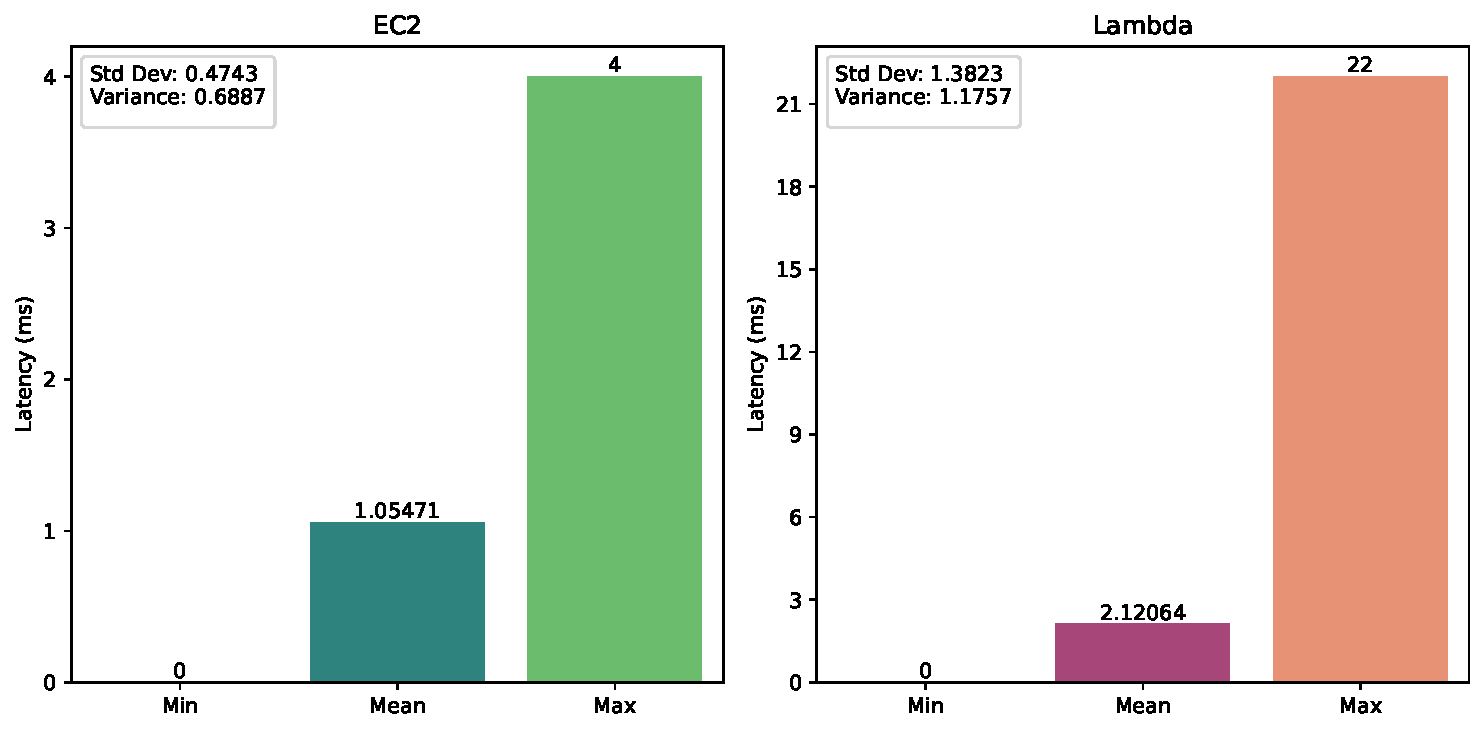
\includegraphics[width=\linewidth]{./fig/bar-rds-constant.pdf}
		\caption{Constant Workload on RDS}
		\label{fig:bar_rds_const}
	\end{subfigure}
	\hfill
	\begin{subfigure}{0.49\linewidth}
		\centering
		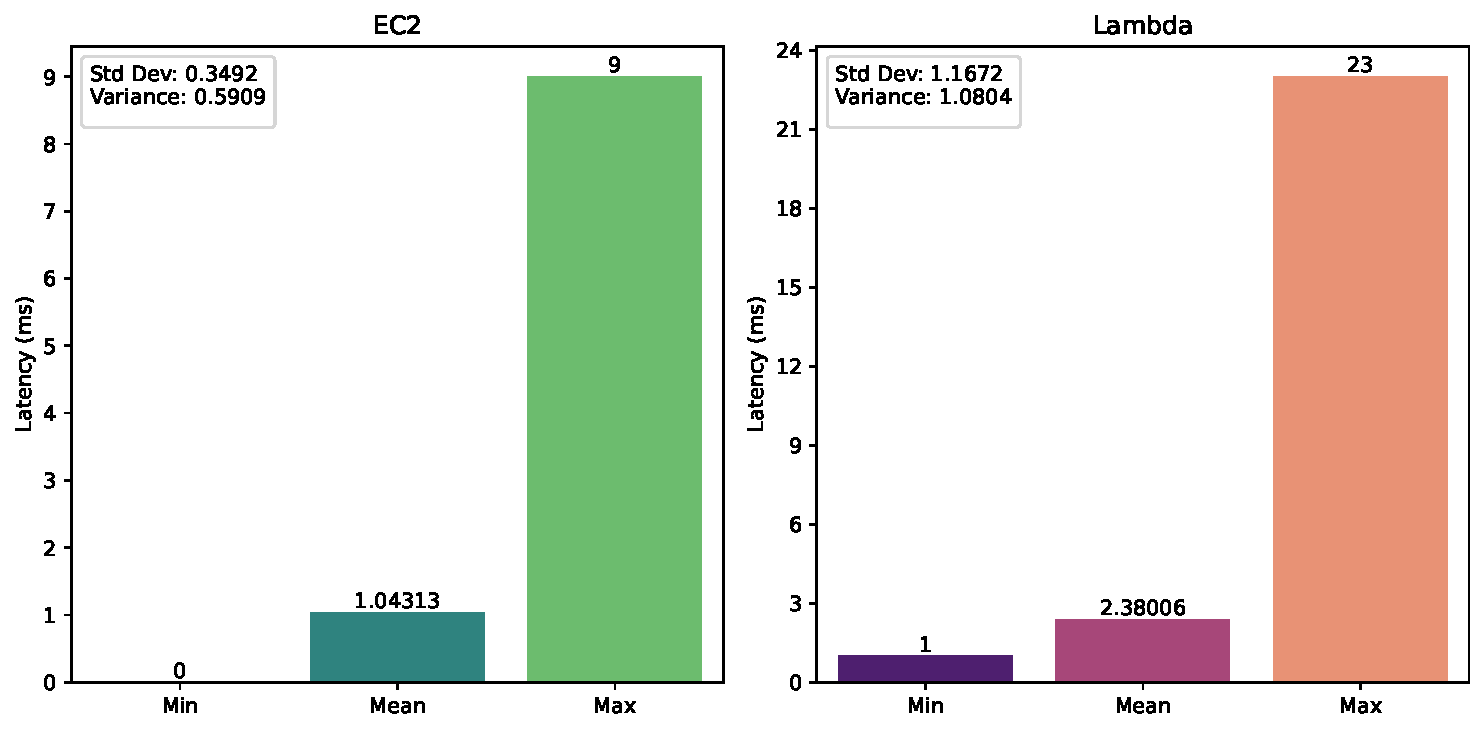
\includegraphics[width=\linewidth]{./fig/bar-rds-bursty.pdf}
		\caption{Burst Workload on RDS}
		\label{fig:bar_rds_bursty}
	\end{subfigure}
	\vfill
	\begin{subfigure}{0.49\linewidth}
		\centering
		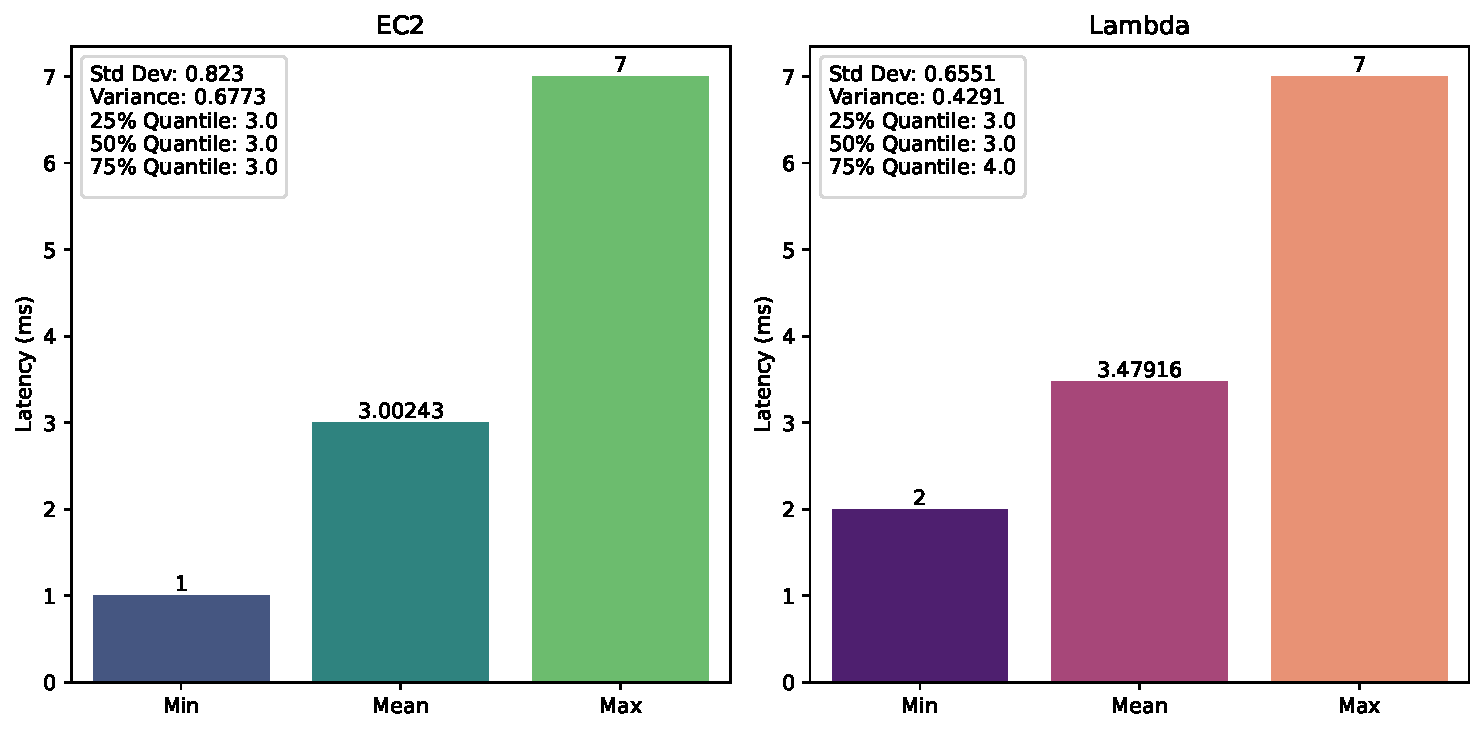
\includegraphics[width=\linewidth]{./fig/bar-dynamo-constant.pdf}
		\caption{Constant Workload on DynamoDB}
		\label{fig:bar_ddb_const}
	\end{subfigure}
	\hfill
	\begin{subfigure}{0.49\linewidth}
		\centering
		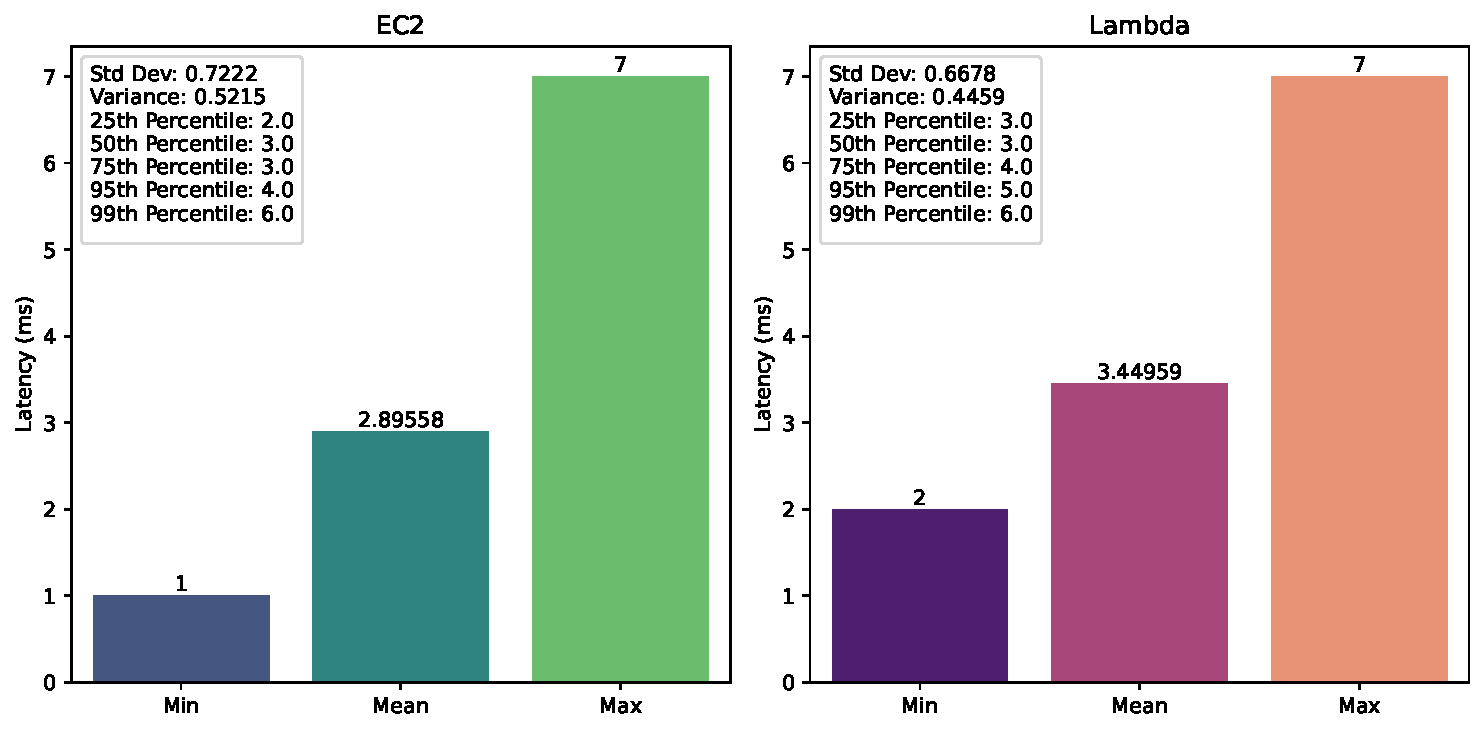
\includegraphics[width=\linewidth]{./fig/bar-dynamo-bursty.pdf}
		\caption{Burst Workload on DynamoDB}
		\label{fig:bar_ddb_bursty}
	\end{subfigure}
	\vfill
	\begin{subfigure}{0.49\linewidth}
		\centering
		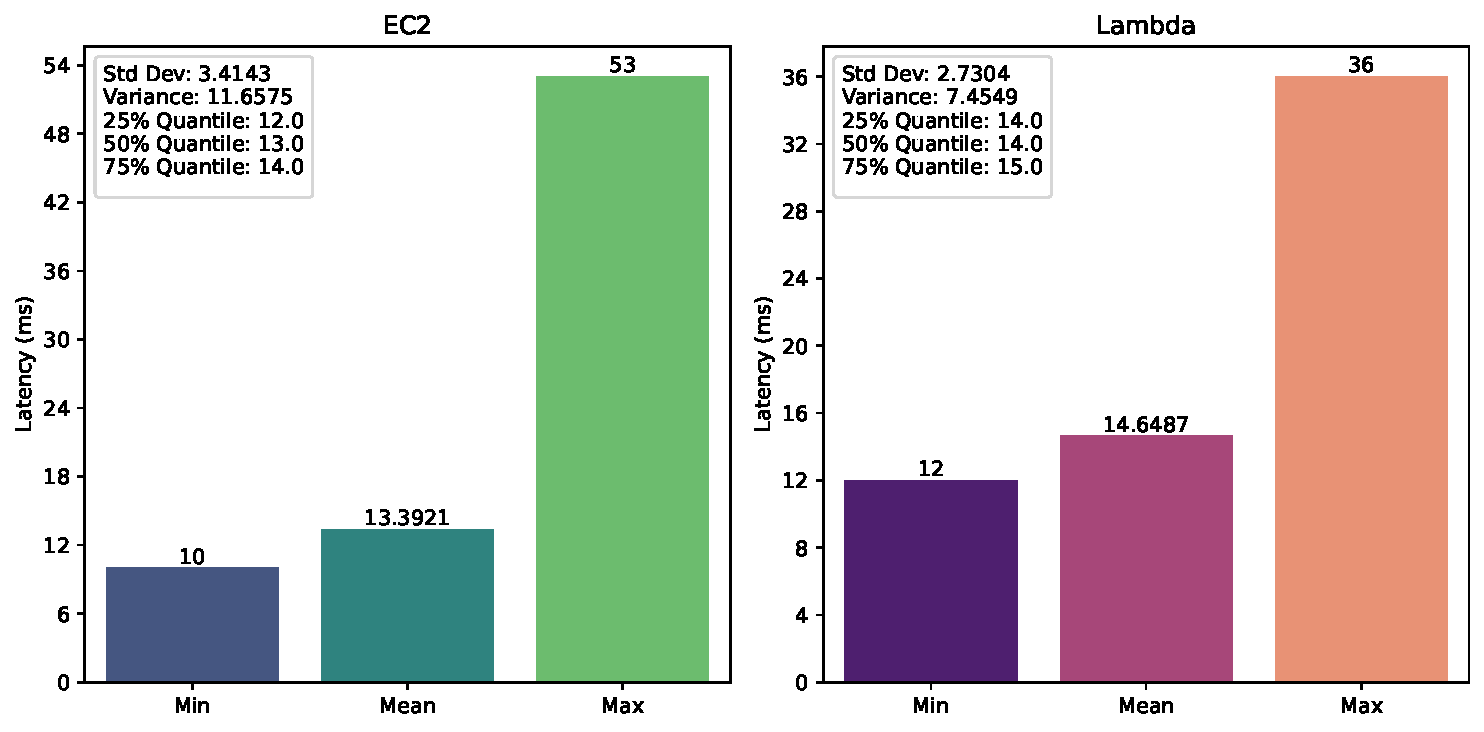
\includegraphics[width=\linewidth]{./fig/bar-s3-constant.pdf}
		\caption{Constant Workload on S3}
		\label{fig:bar_s3_const}
	\end{subfigure}
	\hfill
	\begin{subfigure}{0.49\linewidth}
		\centering
		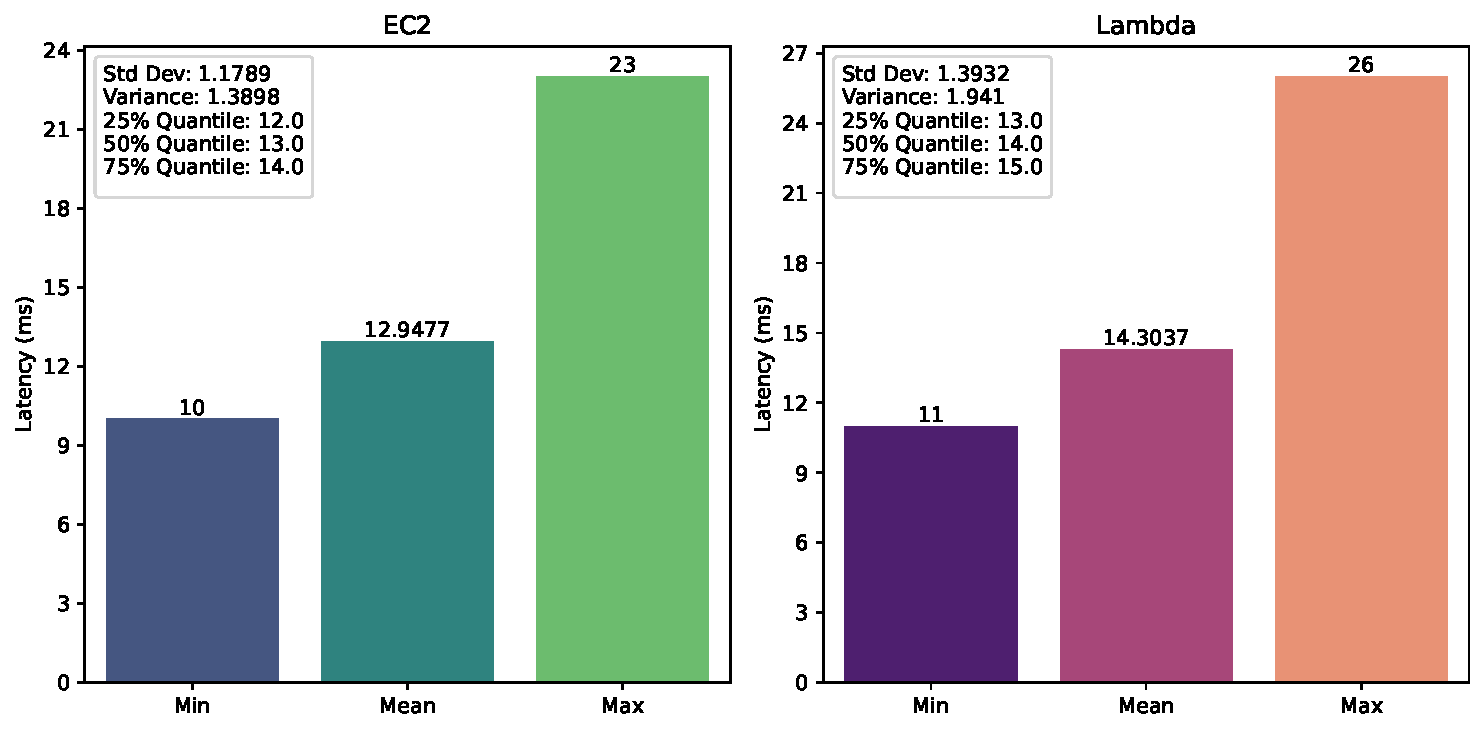
\includegraphics[width=\linewidth]{./fig/bar-s3-bursty.pdf}
		\caption{Burst Workload on S3}
		\label{fig:bar_s3_bursty}
	\end{subfigure}
	\caption{Aggregation of Latency Measurements}
	\label{fig:bar-plots}
\end{figure}

\begin{figure}[h]
	\begin{subfigure}{0.49\linewidth}
		\centering
		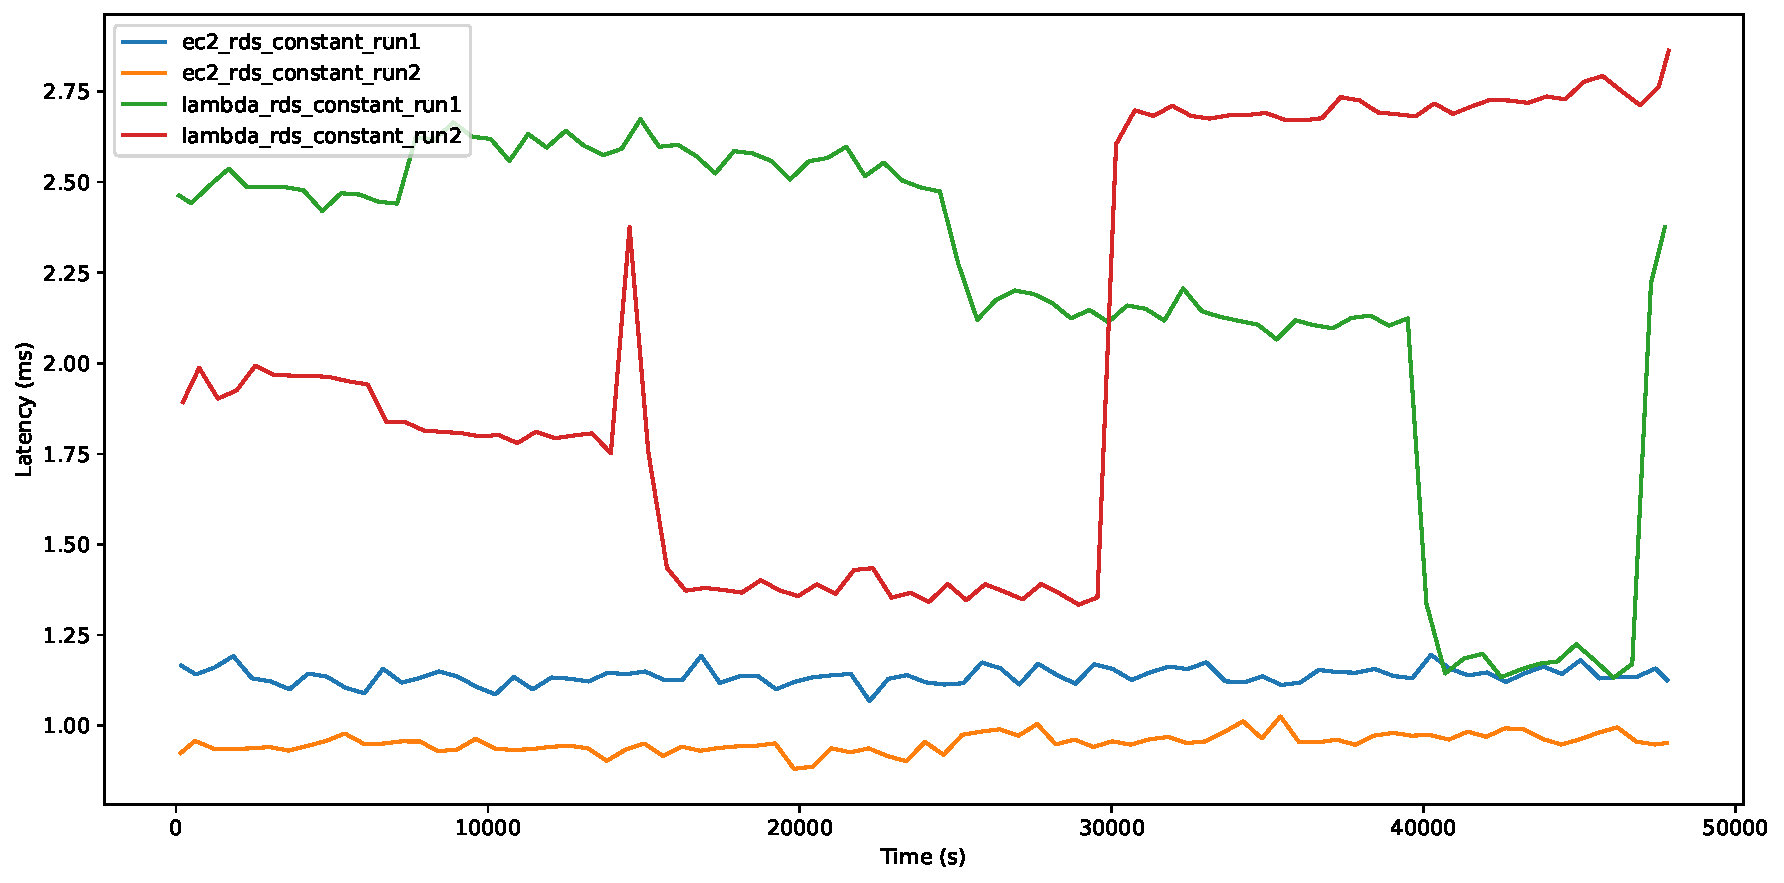
\includegraphics[width=\linewidth]{./fig/ts-rds-constant.pdf}
		\caption{Constant Workload on RDS}
		\label{fig:ts_rds_const}
	\end{subfigure}
	\hfill
	\begin{subfigure}{0.49\linewidth}
		\centering
		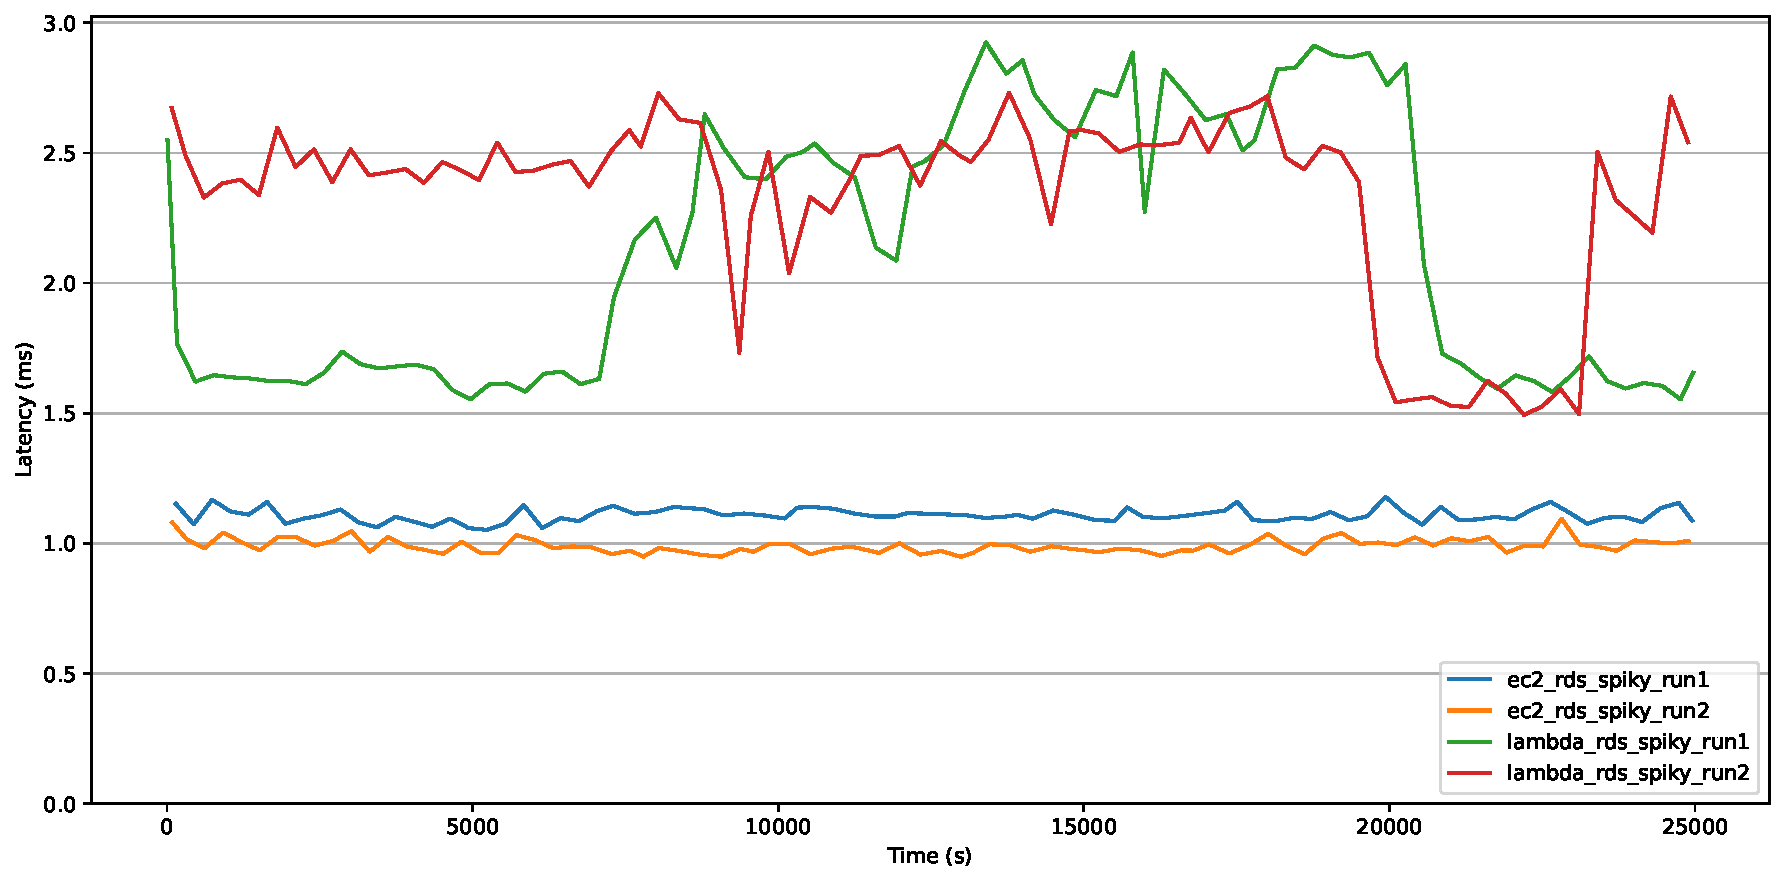
\includegraphics[width=\linewidth]{./fig/ts-rds-bursty.pdf}
		\caption{Burst Workload on RDS}
		\label{fig:ts_rds_bursty}
	\end{subfigure}
	\vfill
	\begin{subfigure}{0.49\linewidth}
		\centering
		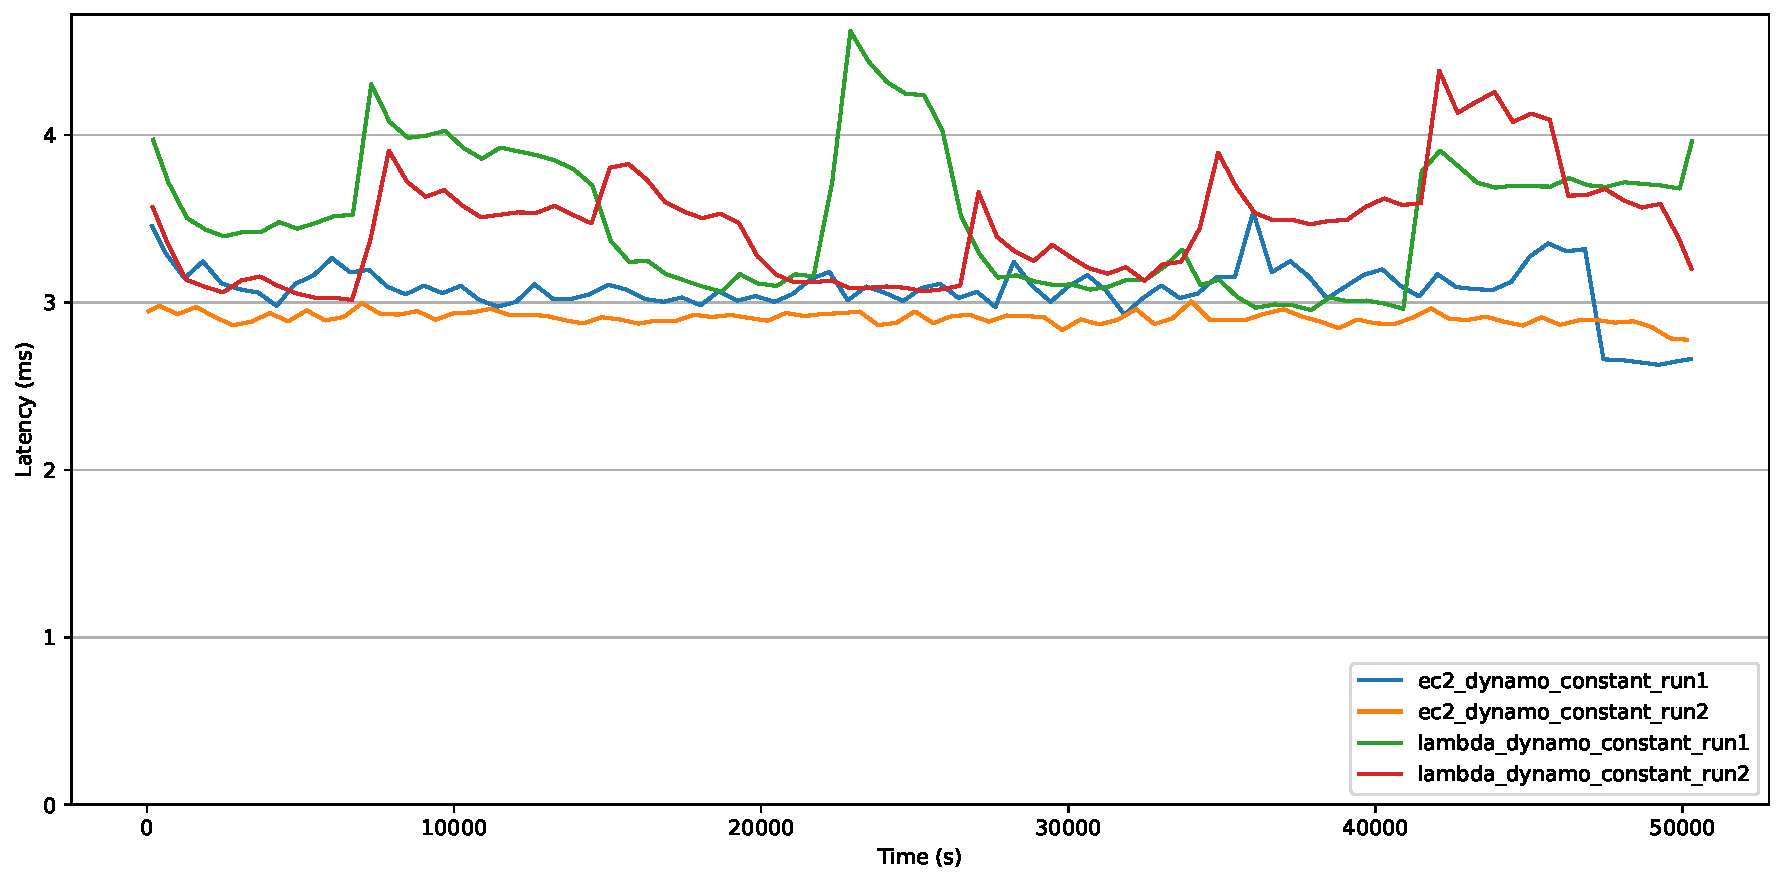
\includegraphics[width=\linewidth]{./fig/ts-dynamo-constant.pdf}
		\caption{Constant Workload on DynamoDB}
		\label{fig:ts_ddb_const}
	\end{subfigure}
	\hfill
	\begin{subfigure}{0.49\linewidth}
		\centering
		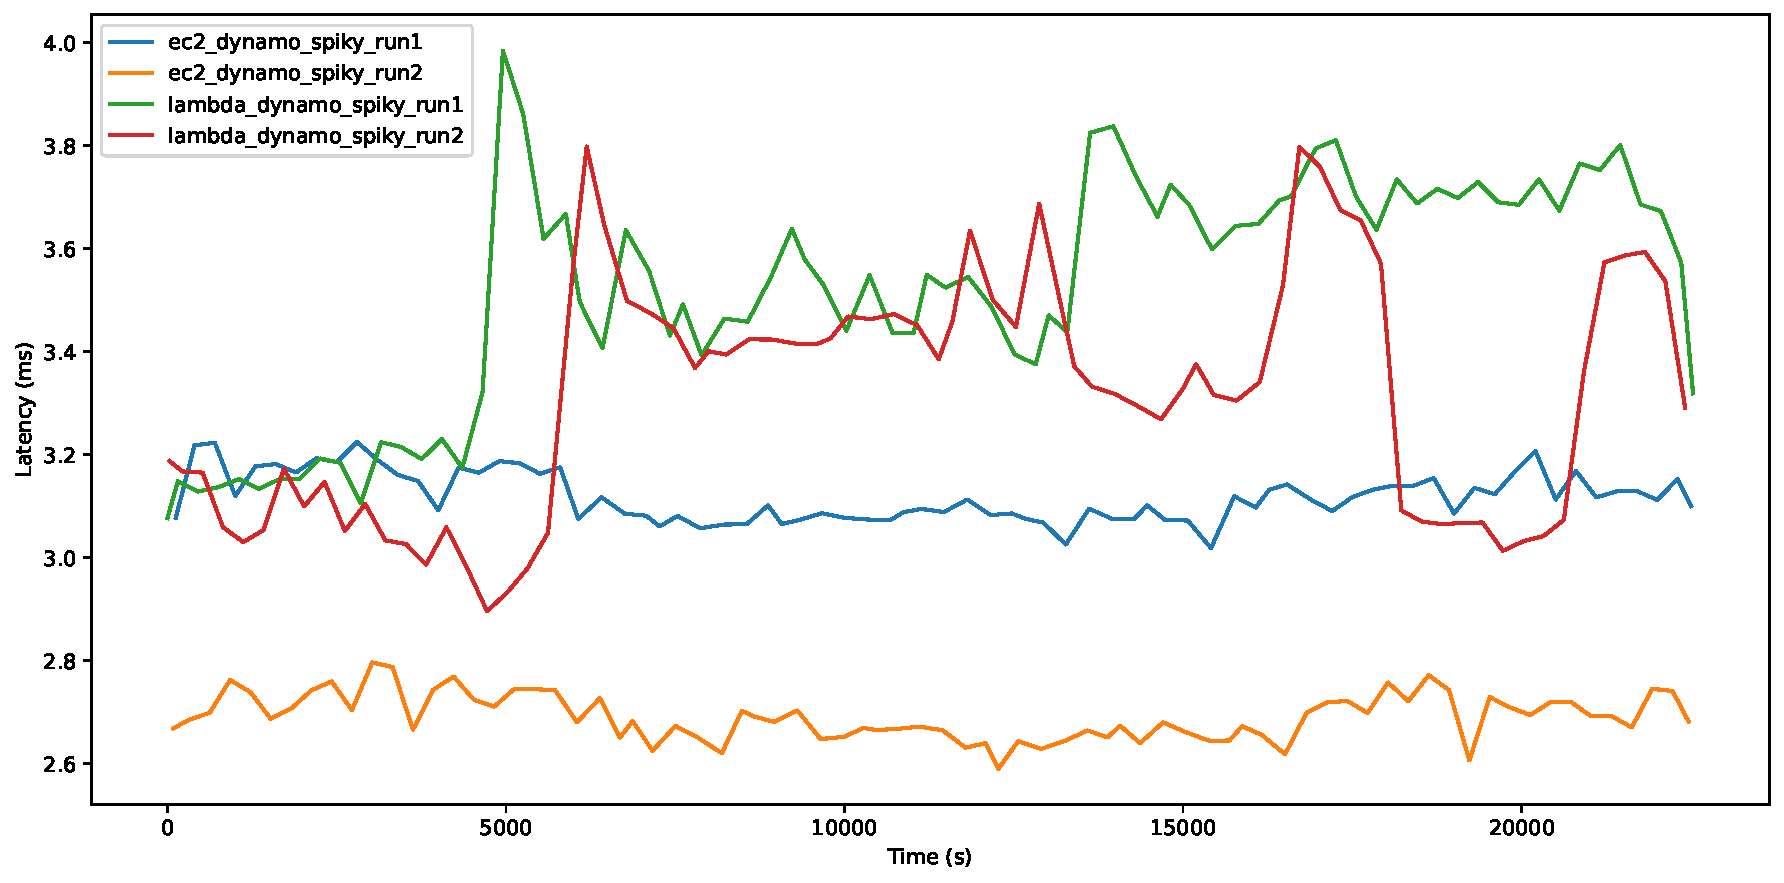
\includegraphics[width=\linewidth]{./fig/ts-dynamo-bursty.pdf}
		\caption{Burst Workload on DynamoDB}
		\label{fig:ts_ddb_bursty}
	\end{subfigure}
	\vfill
	\begin{subfigure}{0.49\linewidth}
		\centering
		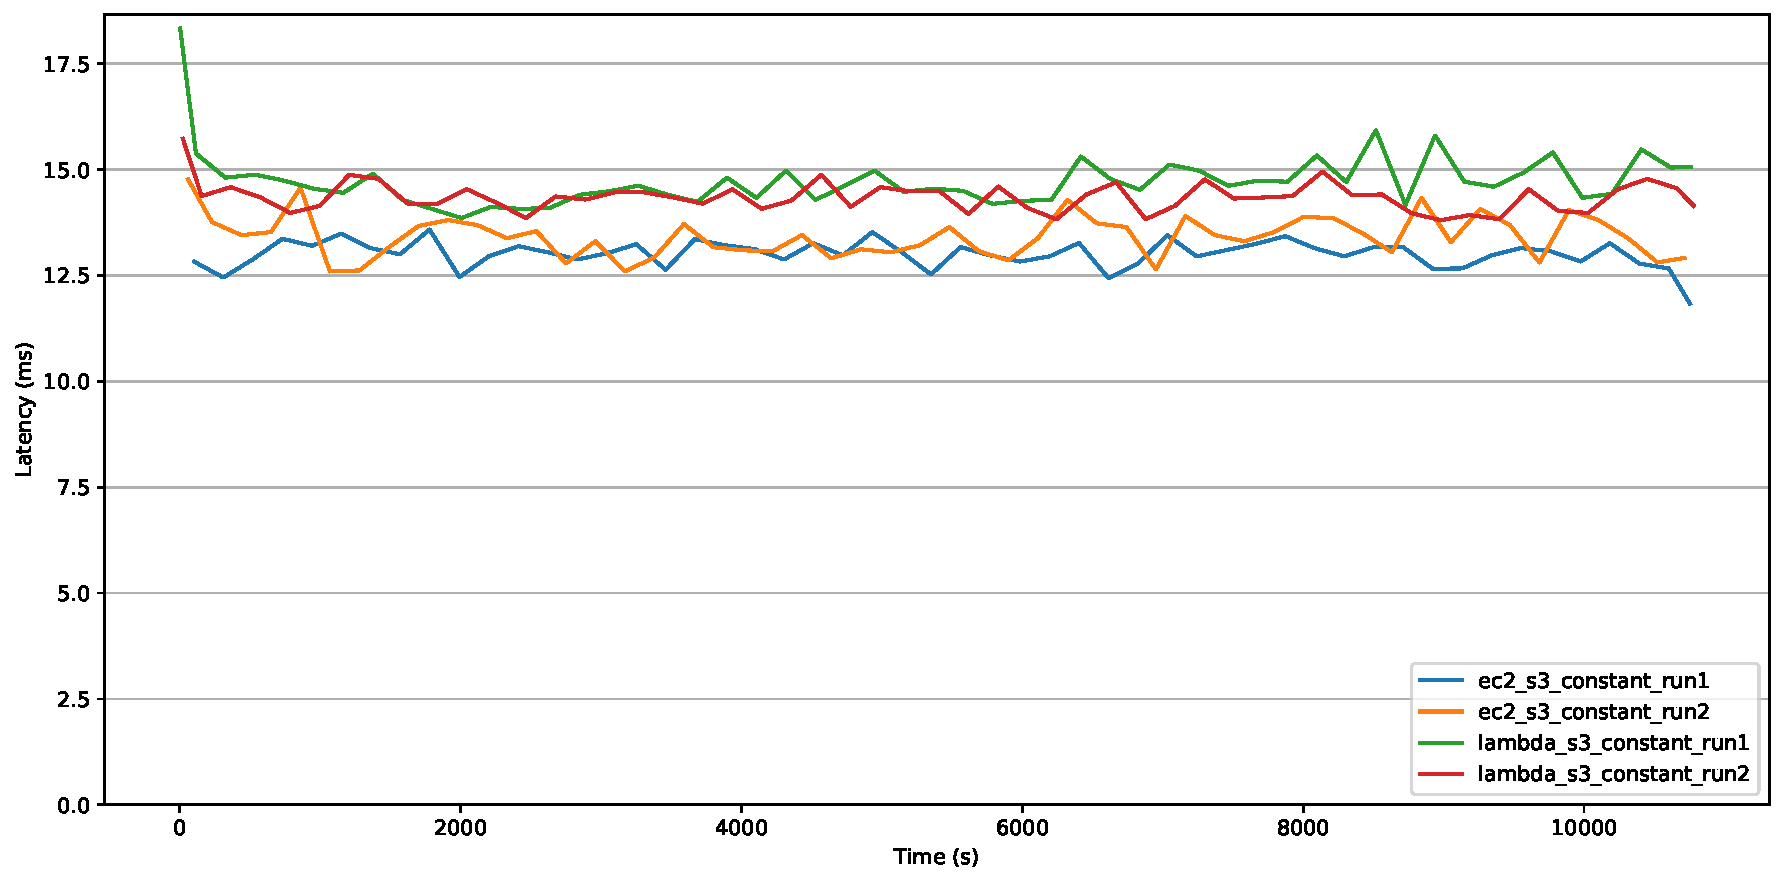
\includegraphics[width=\linewidth]{./fig/ts-s3-constant.pdf}
		\caption{Constant Workload on S3}
		\label{fig:ts_s3_const}
	\end{subfigure}
	\hfill
	\begin{subfigure}{0.49\linewidth}
		\centering
		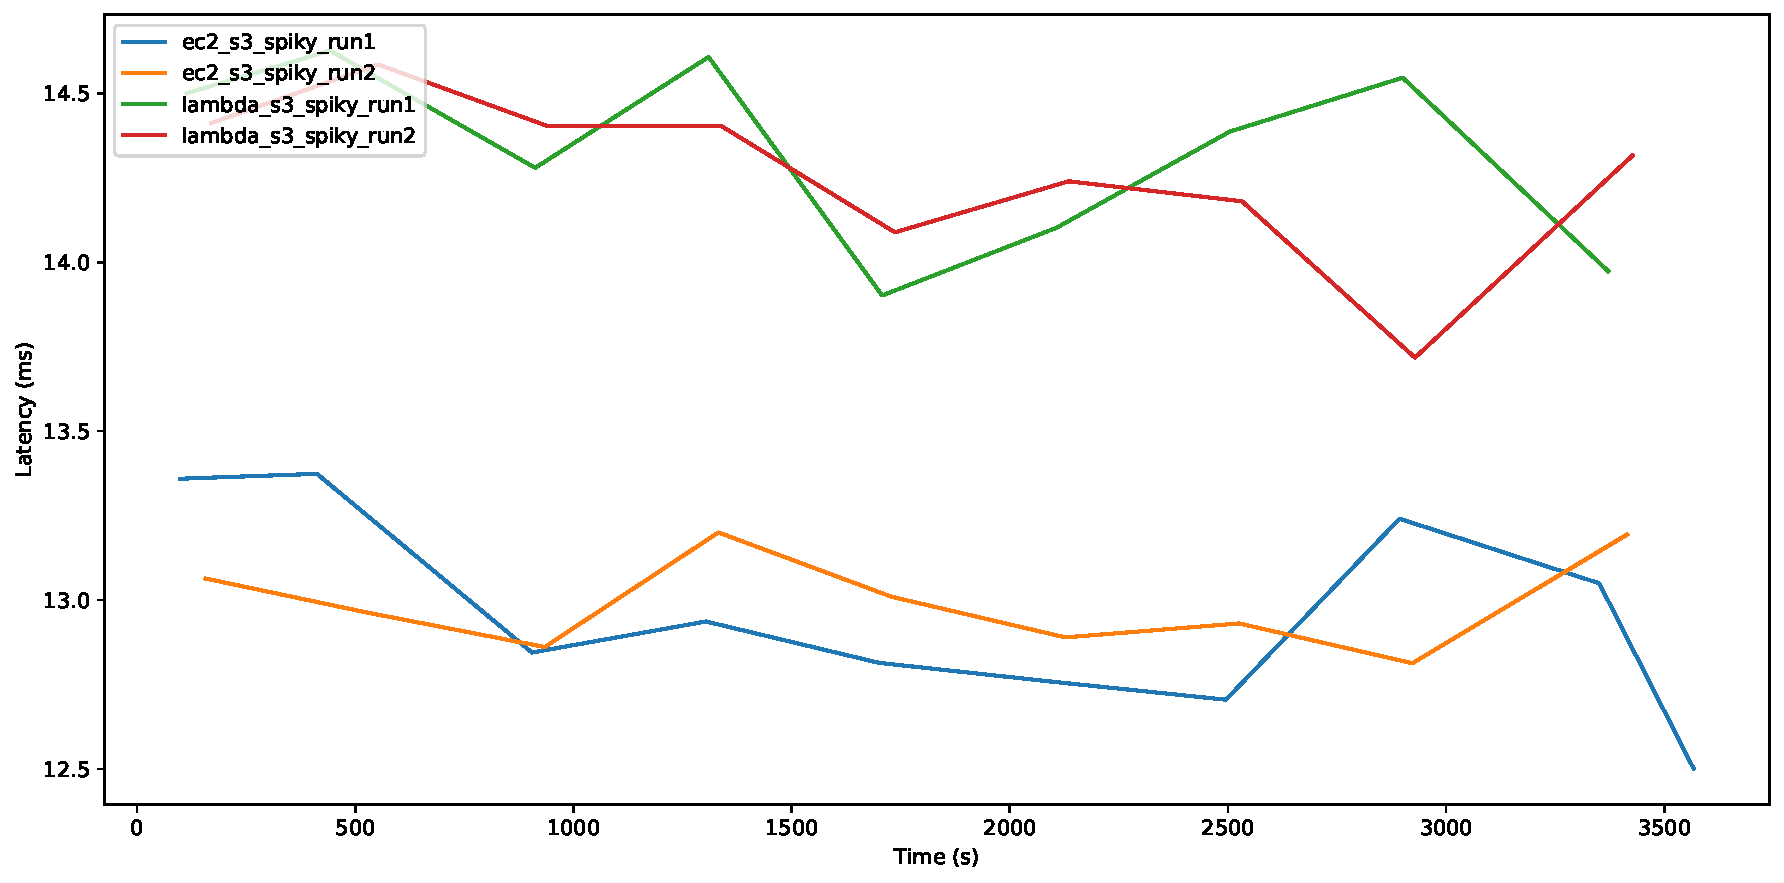
\includegraphics[width=\linewidth]{./fig/ts-s3-bursty.pdf}
		\caption{Burst Workload on S3}
		\label{fig:ts_s3_bursty}
	\end{subfigure}
	\caption{Time-Series Representation of Latency Measurements}
	\label{fig:ts-plots}
\end{figure}


\clearpage
\section{Discussion}
\label{cha:discuss}

This study evaluated latency performance between AWS compute service and datastore pairs. The findings indicate latency trends influenced by compute-service choice and workload characteristics. However, several aspects of the methodology and limitations must be critically analyzed to contextualize these outcomes.

This study encountered several significant limitations. The constraints of the AWS Free Tier restricted the duration and scale of experiments, limiting the observation of long-term performance trends. The reliance on low-tier configurations, such as t3.micro instances, prevented evaluation in realistic production environments where higher-capacity instances are standard. Temporal variability in cloud performance was another challenge, with short-duration benchmarks potentially not capturing the real distribution of the latency metric caused by time-of-day effects or transient network conditions. Additionally, the absence of multi-region setups meant geo-distributed latency behaviors were not analyzed. Simplified use cases focusing on read operations excluded mixed read-write workloads and asynchronous interactions, which are typical in production systems. Lastly, while statistical methods effectively identified and excluded outliers, their underlying causes were not investigated, leaving critical insights into rare performance anomalies unaddressed.

This study's findings indicate implications for designing cloud-based systems. EC2 pairs consistently demonstrated lower access latency, making it a reliable choice for applications with high-performance requirements. However, the relatively small differences in latency observed between Lambda and EC2 pairs, particularly with DynamoDB, indicate that Lambda could be a viable option for scenarios where operational simplicity and scalability are prioritized over minimal latency. To build upon these findings, future research should consider more extensive benchmarks involving realistic production configurations, mixed workloads, long-running experiments, and multi-region setups to better understand the dynamics of latency in diverse scenarios.

\clearpage
\section{Related Work}
\label{cha:relatedwork}

Cloud computing is a widely adopted paradigm, resulting in extensive literature exploring various aspects of its ecosystem. Given the scale of cloud applications and architectures, this study falls under the category of micro-benchmarking, where existing work remains relatively limited. Nonetheless, there are overlaps with studies focusing on different but related aspects of cloud performance.

Villamizar et al. \cite{paper_villamizar_lambdaXec2} compare infrastructure costs and performance of web applications deployed using three architectures: Lambda-based microservices, EC2-based microservices, and monolithic. For data storage, they use PostgreSQL on EC2, though it is unclear if RDS is employed. Unlike this thesis, their study measures latency from a web user’s perspective, factoring in variables like gateways, cold starts, load balancing, and internal communication overhead. Their findings indicate that the Lambda-based microservice architecture achieves better average response times for end users.

Klimovic et al. \cite{paper_klimovic_lambdaXs3} evaluate the suitability of storage options for serverless analytics, including S3, Redis\footcite{https://redis.io/}, and Crail-ReFlex\footcite{https://craillabs.github.io/}, to address ephemeral data sharing requirements. They highlight the overhead of using S3 for latency-sensitive serverless applications, identifying Redis as a lower-latency alternative. Their study examines latency between AWS Lambda and S3 for both read and write operations, reporting $12.1ms$ read and $25.8ms$ write latency for $1KB$ requests. Additionally, they analyze aspects like I/O time, throughput, job runtime, and concurrency.

Palepu et al. \cite{paper_palepu_lambdaXs3ddb} benchmark data transfer rates across serverless and datastore services, including AWS Lambda, S3, and DynamoDB. They identify factors affecting performance, such as memory allocation and concurrency, and highlight Lambda's limitations in scaling data transfer rates under high concurrency. The study reports that Lambda exhibits lower throughput with S3 and DynamoDB compared to EC2 but does not provide specific latency insights.

Albuquerque-Junior et al. \cite{paper_albu_lambdaec2} benchmark AWS Lambda against AWS Beanstalk \footcite{https://aws.amazon.com/elasticbeanstalk/}, which is based on EC2 instances, to evaluate performance in microservice architectures. They use PostgreSQL for data persistence, but it is unclear whether it is RDS. Unlike our approach, they focus on end-to-end performance using a closed workload model, with experiments lasting just over 4 minutes and an unspecified number of repetitions. There are fairness concerns due to the resource configuration: Lambda is allocated $256MB$ of memory ($0.167vCPU$), while Beanstalk uses a t1.micro EC2 instance with $1vCPU$ and $0.613GB$ of memory. They also examine the impact of resource allocation and service configuration. Their results show that EC2 with Beanstalk outperforms Lambda in terms of both read and write latencies.

\clearpage
\section{Conclusion}
\label{cha:conclusion}

Cloud computing has experienced rapid growth, becoming integral to industries seeking scalable and flexible solutions. AWS has emerged as a leader, offering diverse services for computing and storage. Despite its significance, limited empirical data exists on the latency characteristics of AWS compute-datastore interactions, necessitating this study to bridge the knowledge gap.

This thesis investigated the latency performance between AWS compute and datastore service pairs, specifically EC2 and Lambda paired with RDS, DynamoDB, and S3. A systematically conducted benchmark evaluated each pair under constant and burst workloads. Results indicated that EC2 pairs consistently demonstrated lower latency compared to Lambda pairs.

The study highlighted the influence of computing service choices on latency performance and provided empirical data to support architectural decisions in cloud environments. Despite limitations, such as the constraints of AWS Free Tier and the exclusion of mixed workload scenarios, the findings offer foundational insights into the dynamics of service interactions in AWS.

Future work can expand on these results by exploring higher-tier configurations, multi-region setups, and mixed read-write workloads to provide a more comprehensive understanding of cloud service latency characteristics.



\newpage
\printbibliography
\end{document}
